\setcounter{section}{2}

\section{Домашнє завдання за 9/14}

\begin{problem}[1.24, Евграфов]
    Довести, що для довільного додатного $K\ne1$, рівняння $\left\|\dfrac{z-z_1}{z-z_2}\right\|=K$ є рівнянням кола, а також знайдіть центр і радіус цього кола 
\end{problem}

\begin{side_comment}
    На жаль, середньостатистичний читач цього документу не є учасником олімпіад з математики і не знає, що таке коло Аполонія, тому доведеться все доводити.    
\end{side_comment}

\begin{solution}
    Розглянемо точки $z_3$, $z_4$ на прямій $z_1z_2$ для яких $\left\|\dfrac{z_3-z_1}{z_3-z_2}\right\|=K$ і $\left\|\dfrac{z_4-z_1}{z_4-z_2}\right\|=K$. Тоді, за властивістю внутрішньої і зовнішньої бісектрис, $\ell(z.z_3)$ і $\ell(z,z_4)$ є бісектрисами кута $\angle(z_1,z,z_2)$, звідки $\angle(z_3, z, z_4) = 90^\circ$, тобто всі шукані точки $z$ лежать на колі з діаметром $(z_3,z_4)$.\\
    
    Для знаходження радіусу і центру знайдемо $z_3$ і $z_4$ із співвідношень $z_3 - z_1 = K (z_2 - z_3)$ і $z_4 - z_1 = K(z_4 - z_2)$ (тут ми без обмеження загальності вважаємо що $K > 1$): $z_3 = \dfrac{Kz_2 + z_1}{1 + K}$, $z_4 = \dfrac{z_1 - Kz_2}{1 - K}$, звідки $R = \dfrac{\|z_3 - z_4\|}{2} = \dfrac{K}{K^2 - 1}\|z_1 - z_2\|$, а $O = \dfrac{z_3 + z_4}{2} = \dfrac{z_1 + K^2 z_2}{1 - K^2}$.
\end{solution}


\begin{problem}[1.25.1, Евграфов]
    Знайти всі розв'язки наступних систем рівнянь:
    % \begin{enumerate}
        % \item 
        \begin{equation*}
        \left\{
        \begin{aligned}
            \left\| \dfrac{z - 12}{z - 8i} \right\| &= \dfrac53, \\ 
            \left\| \dfrac{z - 4}{z - 8} \right\| &= 1.
        \end{aligned}
        \right.
        \end{equation*} 
        %\item $\begin{cases} \|z^2 - 2i\| = 4, \\ \left\| \dfrac{z + 1 + i}{z - 1 - i} \right\| = 1. \end{cases}$
    % \end{enumerate}
\end{problem}

\begin{solution}
    Нехай $z = x + iy$, тоді перше рівняння переписується наступним чином:
    \[ \left\| \dfrac{(x - 12) + iy}{x + i(y - 8)} \right\| = \dfrac53. \]
    Враховуючи, що $\left\| \dfrac{z_1}{z_2} \right\| = \dfrac{\| z_1 \|}{\| z_2 \|}$, отримуємо
    \[ 3 \|(x - 12) + iy\| = 5 \|x + i(y - 8)\|. \]
    Далі, за визначенням норми комплексного числа маємо
    \[ 9 (x^2 - 24 x + 144 + y^2) = 25 (x^2 + y^2 - 16 y + 64). \]
    З другого рівняння системи аналогічним чином знаходимо
    \[ x^2 - 8x + 16 + y^2 = x^2 - 16 x + 64 + y^2 , \]
    звідки $8x = 48$ і $x = 6$. Підставляючи це у перше рівняння, знаходимо
    \begin{equation*}
    \begin{aligned}
    9 (36 - 144 + 144 + y^2) &= 25 (36 + y^2 - 16 y + 64) \\
    324 + 9 y^2 &= 2500 + 25 y^2 - 400 y \\
    0 &= 16 y^2 - 400 y + 2176 \\
    324 &= (4 y - 50)^2 \\
    \pm 18 &= 4 y - 50 \\
    y_{1, 2} &= 8, 17
    \end{aligned}
    \end{equation*}
    Тобто, остаточна відповідь $z_1 = 6 + 8i$, $z_2 = 6 + 17i$.
\end{solution}

\begin{problem}[1.43, Евграфов]
    При яких значеннях параметра $a > 0$ наступні кола комплексної площини відповідають великим колам на сфері Рімана:
    \begin{enumerate}
        \item $\| z - a \| = a$;
        \item $\left \| z + \dfrac a 2 \right \| = a$;
        \item $\| z - i \| = a$;
        \item $\| z - 2 a i \| = a$.
    \end{enumerate}
\end{problem}

\begin{solution}
    \begin{enumerate}
        \item Зауважимо, що $z = 0$ лежить на цьому колі комплексної площини, а всі великі кола сфери Рімана які містять 0 містять ще й $\infty$, протиріччя, тобто таких $a$ не існує.
        \begin{side_comment}
            Або можна сказати що нам підійде $a = \infty$, але це трохи нечесно у плані введення арифметичних операції з нескінченністю.
        \end{side_comment}
        \item Розглянемо точки $z_1 = a / 2$ і $z_2 = - 3 a / 2$, вони мають перейти у діаметрально протилежні точки сфери Рімана.
        \[\xi_1 = \dfrac {2 a} {4 + a^2}, \quad \xi_2 = -\dfrac{6 a}{4 + 9 a^2}, \quad \eta_1 = \eta_2 = 0, \quad \stigma_1 = \dfrac{a^2}{4 + a^2}, \quad \stigma_2 = \dfrac{9 a^2}{4 + 9 a^2}.\]
        Точки з такими координатами є діаметрально протилежними якщо 
        \[ \dfrac {2 a} {4 + a^2} = \xi_1 = - \xi_2 = \dfrac{6 a}{4 + 9 a^2} \quad \text{та} \quad 1 = \stigma_1 + \stigma_2 = \dfrac{a^2}{4 + a^2} + \dfrac{9 a^2}{4 + 9 a^2}, \]
        звідки $a = 2 / \sqrt 3$.
        \item Розглянемо точки $z_1 = i + a i $ і $z_2 = i - a i$, вони мають перейти у діаметрально протилежні точки сфери Рімана.
        \[\xi_1 = \xi_2 = 0, \quad \eta_1 = \dfrac{1 + a}{1 + (1 + a)^2}, \quad \eta_2 = \dfrac{1 - a}{1 + (1 - a)^2}, \quad \stigma_1 = \dfrac{(1 + a)^2}{1 + (1 + a)^2}, \quad \stigma_2 = \dfrac{(1 - a)^2}{1 + (1 - a)^2}.\]
        Точки з такими координатами є діаметрально протилежними якщо 
        \[ \dfrac{1 + a}{1 + (1 + a)^2} = \eta_1 = - \eta_2 = \dfrac{a - 1}{1 + (1 - a)^2} \quad \text{та} \quad 1 = \stigma_1 + \stigma_2 = \dfrac{(1 + a)^2}{1 + (1 + a)^2} + \dfrac{(1 - a)^2}{1 + (1 - a)^2},\]
        звідки $a = \sqrt 2$.
        \item $\forall a$ $\| 0 - 2ai \| = 2a > a$, тобто коло (круг) на площині не містить (всередині) точки 0, тому відповідне коло на сфері Рімана точно не є великим (хоча би тому що воно повністю лежить в одній напівсфері).
    \end{enumerate}
\end{solution}

\begin{problem}[1.45, Евграфов]
    Дати геометричний опис множин точок $z$ комплексної площини, що задовольняють нерівностям:
    \begin{enumerate}
        \item $k(z, 0) < R$, $0 < R < 1$;
        \item $k(z, \infty) < R$, $0 < R < 1$;
        \item $k(z, i) > \dfrac 1 {\sqrt 2}$;
        \item $\dfrac 1 2 < k(z, 1) < \dfrac 1 {\sqrt 2}$.
    \end{enumerate}
    Тут $k(z_1, z_2) = d(M(z_1), M(z_2))$ -- звичайна Евклідова (хордальна) відстань у просторі $\RR^3$.
\end{problem}

\begin{solution}
    \begin{enumerate}
        \item З $\triangle(0, M(z), \infty)$: 
        \[ d(0, M(z)) < R \Rightarrow d(\infty, M(z)) > \sqrt {1 - R^2}.\]
        Як відомо з курсу шкільної геометрії, 
        \[ d(0, M(z)) = \sqrt{d(z, M(z)) \cdot d(M(z), \infty)}, \]
        тому 
        \[ d(z, M(z)) = d^2(0, M(z)) / d(M(z), \infty) < R^2 / \sqrt{1 - R^2}. \]
        Далі,
        \[ d(0, z) = \sqrt{d^2(0, M(z)) + d^2(M(z), z)} < \sqrt{R^2 + R^4 / (1 - R^2)} = R / \sqrt{1 - R^2}, \]
        звідки описом відповідної множини у комплексній площині буде $B_{R / \sqrt{1 - R^2}}(0)$.
        \item
        Поєднуючи результат попереднього пункту і здоровий глузд, отримуємо $\CC \setminus B_{\sqrt{1 - R^2}/R}(0)$.
        \item Враховуючи, що точка $i$ переходить на ``екватор'' сфери Рімана, і той факт, що $d(i, \infty) = d(i, 0) = 1 / \sqrt{2}$, отримуємо півплощину $\Imag z < 0$.
        \item З попереднього пункту, $k(z, 1) < 1 / \sqrt 2$ задає півплощину $\Real z > 0$, а $k(z, 1) > 1 / 2$ виключає з неї якийсь круг, а саме $B_{\sqrt 5}(2)$ (визначається по двом діаметрально протилежним точкам).
    \end{enumerate}
\end{solution}

\begin{problem}[1.55, Волковиський]
    Довести, що при стереографічній проекції кути між кривими на сфері дорівнюють кутам між їхніми образами на площині.
\end{problem}

\begin{solution}
    Нехай $M$ -- довільна, відмінна від полюса $P$ точка на сфері Рімана, а $\gamma_1$ та $\gamma_2$ -- неперервні криві на сфері, які проходять через точку $M$ і мають у ній дотичні. Нехай кут, утворений дотичними, дорівнює $\alpha$. Позначимо через $Z$ точку комплексної площини, яка є образом $M$, а через $\Gamma_1$ та $\Gamma_2$ -- образи кривих $\gamma_1$ та $\gamma_2$ при стереографічному відображенні. Позначимо через $\beta$ кут між дотичними до $\Gamma_1$ та $\Gamma_2$ у точці $Z$. Покажемо, що він дорівнює $\alpha$.\\
    
    \begin{figure}[H]
        \centering
        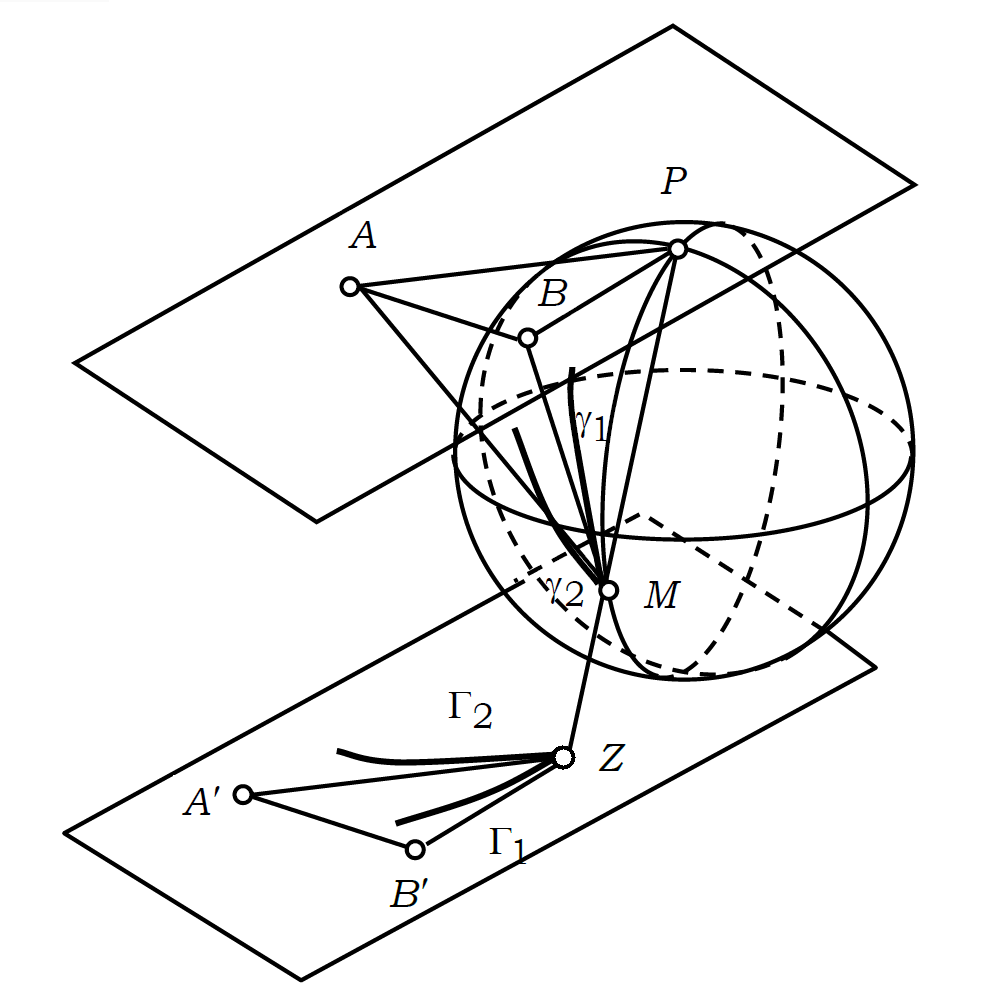
\includegraphics[scale=.321]{55.png}
    \end{figure}
    
    
    % Нехай $M_0(\xi_0, \eta_0, \stigma_0)$ -- довільна, відмінна від полюса $P$ точка на сфері Рімана, а $\gamma_1$ та $\gamma_2$ -- неперервні криві на сфері, які проходять через точку $M_0$ і мають у ній дотичні. Нехай кут, утворений дотичними, дорівнює $\alpha$. Оскільки $\gamma_1$ та $\gamma_2$ -- криві з дотичними, то вони можуть бути задані параметрично за допомогою функції 
    % \[ \xi_k = \phi_k(t), \eta_k = \psi_k(t), \stigma_x=\chi_k(t) \quad (k=1,2),\]
    % які задовольняють рівняння сфери 
    % \[\phi_k^2 + \psi_k^2 + (\chi_k - 1/2)^2 \equiv 1/4,\]
    % диференційовні в точка $t = t_0$ (що відповідає точці $M_0$), а також криві не мають сингулярностей (чи особливих точок якогось там виду, не скажу сходу як вони точно називаються), тобто 
    % \[\forall t \, (\dot \phi_k(t))^2 + (\dot \psi_k(t))^2 + (\dot \chi_k(t))^2 \ne 0.\]
    
    % Позначимо через $Z_0(x_0, y_0)$ точку комплексної площини, яка є образом $M_0$, а через $\Gamma_1$ та $\Gamma_2$ -- образи кривих $\gamma_1$ та $\gamma_2$ при стереографічному відображенні. Тоді координати кривих $\Gamma_1$ та $\Gamma_2$ задаються рівняннями
    % \[ x_k \equiv \dfrac{\xi_k}{1 - \stigma_k} \equiv \dfrac{\phi_k}{1 - \chi_k}, \quad y_k \equiv \dfrac{\eta_k}{1 - \stigma_k} \equiv \dfrac{\psi_k}{1 - \chi_k} \quad (k = 1, 2). \]
    
    % Оскільки $M_0 \ne P$, то $\stigma_k(0) \ne 1$, тобто $\chi_k(t_0) \ne 1$, звідки $1 - \chi_k(t_0) \ne 0$, тобто координати точок кривих $\Gamma_k$ скінченні (принаймні у деякому околі $M_0$, а тому цілком законно можна розглянути $\dot x_k(t_0)$ та $\dot y_k(t_0)$:
    % \[ \dot x_k(t_0) = \left(\dfrac{\xi_k}{1 - \stigma_k}\right)^\prime(t_0) = \dfrac{\dot \xi_k(t_0) (1 - \stigma_k(t_0)) + \dot \stigma_k(t_0) \xi_k(t_0)}{(1 - \stigma_k(t_0))^2}\]
    % \[ \dot y_k(t_0) = \left(\dfrac{\eta_k}{1 - \stigma_k}\right)^\prime(t_0) = \dfrac{\dot \eta_k(t_0) (1 - \stigma_k(t_0)) + \dot \stigma_k(t_0) \eta_k(t_0)}{(1 - \stigma_k(t_0))^2}\]
    
    Для цього продовжимо дотичні до сферичних кривих до перетину їх з дотичною площиною до сфери в точці $P$. Розглянемо трикутники $\triangle APB$ та $\triangle AMB$. Оскільки $AB$ -- спільна сторона обох трикутників, $AP = AM$ та $BP = BM$ як дотичні до кола, що виходять з однієї точки, то трикутники $\triangle APB$ та $\triangle AMB$ рівні між собою. Отже, $\angle APB = \angle AMD = \alpha$. Разом із тим, дотичні до проекцій кривих паралельні прямим $AP$ та $BP$, оскільки ці дотичні є прямими, утвореними перетином площин $PAM$ і $PBM$ із площиною проекцій. Отже, кут між ними дорівнює $\angle APB = \alpha$, тобто $\alpha = \beta$.
\end{solution}